\documentclass[border=6pt]{standalone}
\usepackage{amsmath}
\usepackage{tikz}
\usetikzlibrary{arrows.meta,calc}
\begin{document}
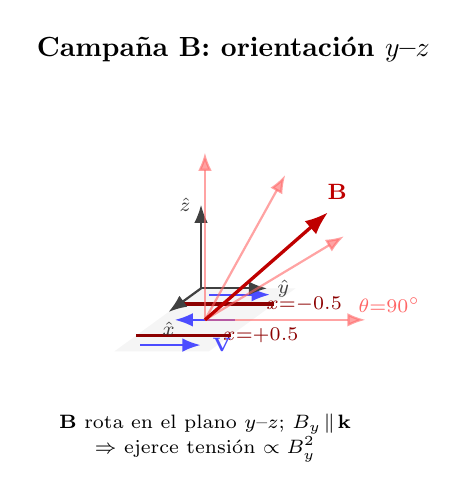
\begin{tikzpicture}[>=Latex,
  Bvec/.style={->,very thick,red!75!black},
  flow/.style={->,blue!70,thick},
  ax/.style={->,thick,black!75}]
\coordinate (O) at (0,0);
\coordinate (px) at (-0.55,-0.40);
\coordinate (py) at (1.20,0);
\coordinate (pz) at (0,1.25);
\newcommand{\PT}[3]{($ (O) + #1*(px) + #2*(py) + #3*(pz) $)}
% --- escena doble-KHI ---
\fill[black!4] \PT{-1}{-0.5}{0} -- \PT{1}{-0.5}{0} -- \PT{1}{0.5}{0} -- \PT{-1}{0.5}{0} -- cycle;
\draw[very thick,red!55!black] \PT{0.5}{-0.5}{0} -- \PT{0.5}{0.5}{0};
\draw[very thick,red!55!black] \PT{-0.5}{-0.5}{0} -- \PT{-0.5}{0.5}{0};
\node[font=\scriptsize,red!55!black] at \PT{0.5}{0.82}{0} {$x{=}{+}0.5$};
\node[font=\scriptsize,red!55!black] at \PT{-0.5}{0.82}{0} {$x{=}{-}0.5$};
\draw[flow] \PT{0}{0.32}{0} -- \PT{0}{-0.32}{0};
\draw[flow] \PT{0.8}{-0.32}{0} -- \PT{0.8}{0.32}{0};
\draw[flow] \PT{-0.8}{-0.32}{0} -- \PT{-0.8}{0.32}{0};
\node[blue!70,font=\scriptsize] at \PT{0.8}{0.55}{0} {$\mathbf V$};
\draw[ax] \PT{-1}{-0.5}{0} -- \PT{-0.25}{-0.5}{0} node[below,font=\scriptsize] {$\hat x$};
\draw[ax] \PT{-1}{-0.5}{0} -- \PT{-1}{0.2}{0} node[right,font=\scriptsize] {$\hat y$};
\draw[ax] \PT{-1}{-0.5}{0} -- \PT{-1}{-0.5}{0.85} node[left,font=\scriptsize] {$\hat z$};
% --- campo: orientacion y-z (rota de z a y) ---
\foreach \t in {0,30,60,90}{
  \pgfmathsetmacro\sy{1.7*sin(\t)}\pgfmathsetmacro\cz{1.7*cos(\t)}
  \draw[->,red!60,opacity=0.6,thick] \PT{0}{0}{0} -- \PT{0}{\sy}{\cz};
}
\pgfmathsetmacro\syb{1.7*sin(50)}\pgfmathsetmacro\czb{1.7*cos(50)}
\draw[Bvec] \PT{0}{0}{0} -- \PT{0}{\syb}{\czb};
\node[red!75!black,font=\footnotesize] at \PT{0}{1.4}{1.3} {$\mathbf B$};
\node[red!60,font=\scriptsize] at \PT{0}{1.95}{0.15} {$\theta{=}90^\circ$};
\node[font=\bfseries] at \PT{0}{0.3}{2.75} {Campaña B: orientación $y$--$z$};
\node[font=\scriptsize,align=center] at \PT{0}{0}{-1.2}
  {$\mathbf B$ rota en el plano $y$--$z$; $B_y\!\parallel\!\mathbf k$\\ $\Rightarrow$ ejerce tensión $\propto B_y^2$};
\end{tikzpicture}
\end{document}
